
\documentclass[main.tex]{subfiles}

\begin{document}


\chapter{Conclusion}

\section{Discussion}
In this project, we reviewed existing instance segmentation technics. We implemented SplineDist. We proposed an improvement to the main architecture by incorporating an overlap branch. The results we observed slightly worse performance than the main paper, but we did not take a subset of the data and used the entirety of the data (as the data contained several modalities). and the data didn't contain much overlap to confirm our hypothesis. further analysis is required.



\section{Conclusion}
The key point to remember from this project are: 
\begin{itemize}
    \item SplineDist achieves better results than Unet alone (+ connected components). 
    \item Spline representation has many benefits and good properties for modeling cells
    \item Increasing the number of control point does not always achieve better results, as it can add more freedom to the model and provide additional noise to the predicted shape.
    \item Incorporating an overlap branch into the model helps the model achieve good results for overlapping cells.
    \item Many tricks were required in order to correctly train the model.
    
\end{itemize}

\section{Further improvement}
\subsection{Different Dataset}
The chosen dataset was poor, it contained eliptical shapes, with relatively no overlap , or in the case of CISD contain only few cells per image (not crowded). a better dataset would contain crowded cells, with variable shapes and scales
\subsection{Multiclass}
SplineDist can be extended for multiclass classification, by adding a probability map for each class, and a softmax layer. we would like to experiment on this point and assert the performance.
\subsection{Better DataAugmentation}
We would like to try different augmentation and measure their importance to the model as we have seen that this 
\subsection{Optimize for memory}
Although the sampling operation is optimized, we still sample all the instances (for each pixel) thus taking up a lot of memory, and with higher number of control points and sample sizes it can become unmanageable. so it's a track to look into.
\subsection{Investigate the patterns observed}
We observed square patterns appearing during the training in the predicted probabilities, we would like to further debug and understand where it was coming from. 
\subsection{3D adaptation}
Several technics exist to adapt the problem of instance segmentation in 3d. We can for instance train a model using the same formulation but instead of B-Spline, we use B-spline surface. for our knowledge, there is no implementation of this approach yet. 

But it requires having 3d Data, which is rare to find in the wild. So another approach is rather reuse a pretrained model on 2d Data. Some common ways to do so:

\begin{itemize}
    \item Apply the 2d model on each slice of the 3d image, then initialize 3d watershed algorithm
    \item Apply the 2d model on each slice of the 3d image, then associate each instance from the slice $t-1$ to its correspondent one in the $t$-th slice. using either a linear assignment, or if a prior knowledge exist, using a Minimum cost Maximum flow (taking consideration of the position of the instance for example). 
\end{itemize}

\begin{figure}[H]
    \centering
    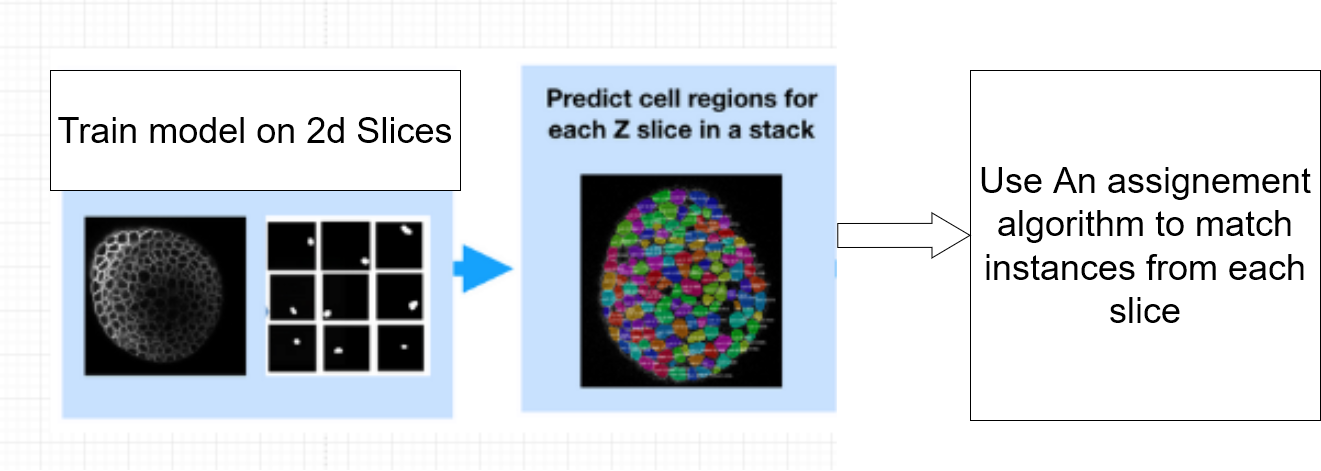
\includegraphics[width=15cm]{presentationImages/slice.png}
    \caption{Exemple of a Procedure to adapt 2d model for 3d images}
\end{figure}

\end{document}
